\documentclass{beamer}
\usepackage[UTF8]{ctex}
\usepackage{graphicx} 
\usepackage{float} 
\usepackage{subfigure}
\usepackage{algorithm,algorithmic}
\usepackage{tikzit}

\input{figs/sample.tikzstyles}
\usetheme{Madrid}
\usecolortheme{default}

%------------------------------------------------------------
%This block of code defines the information to appear in the
%Title page
\title %optional
{基于同构测试的图神经网络简介}

\author % (optional)
{吴钰同}

\date % (optional)
{\today}

%End of title page configuration block
%------------------------------------------------------------



%------------------------------------------------------------
%The next block of commands puts the table of contents at the 
%beginning of each section and highlights the current section:

\AtBeginSection[]
{
  \begin{frame}
    \frametitle{Table of Contents}
    \tableofcontents[currentsection]
  \end{frame}
}
%------------------------------------------------------------


\begin{document}

%The next statement creates the title page.
\frame{\titlepage}


%---------------------------------------------------------
%This block of code is for the table of contents after
%the title page
\begin{frame}
\frametitle{Table of Contents}
\tableofcontents
\end{frame}
%---------------------------------------------------------


\section{Weisfeiler-Lehman Test}

%---------------------------------------------------------
%Changing visivility of the text
\begin{frame}

  \frametitle{图同构}

  \begin{block}{定义}
    对于两个无向图 $G$ 和 $H$,若存在它们顶点之间的双射 $f:V(G) \rightarrow V(H)$,
    使得 $G$ 中的顶点 $u$ 和 $v$ 相邻当且仅当 $H$ 中的顶点 $f(u)$ 和 $f(v)$ 相邻,
    则称 $G$ 和 $H$ 同构。
  \end{block}
  \centering
  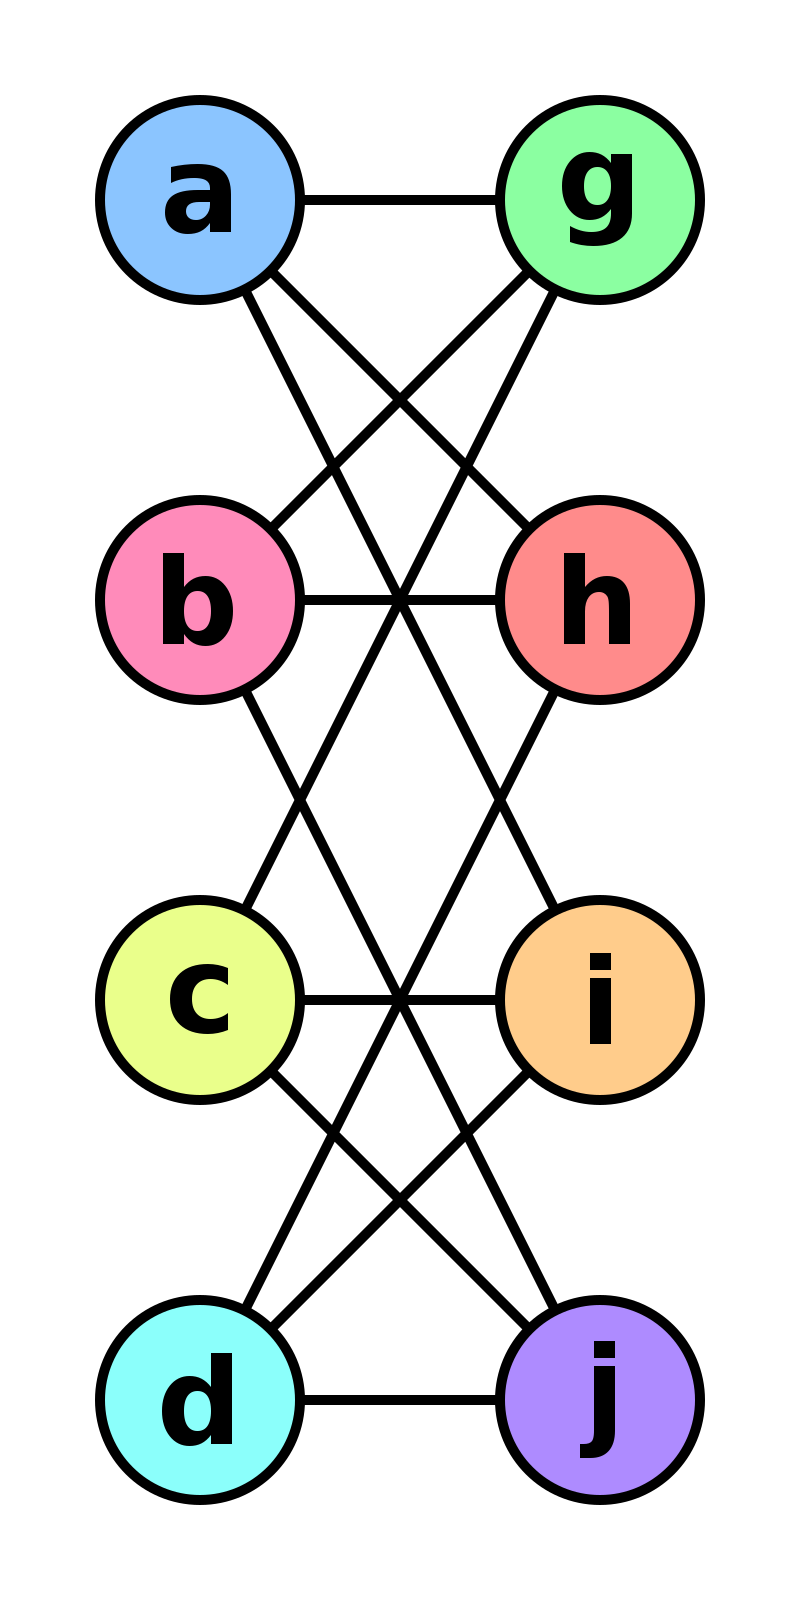
\includegraphics[scale=0.1]{figs/Graph_isomorphism_a.png}
  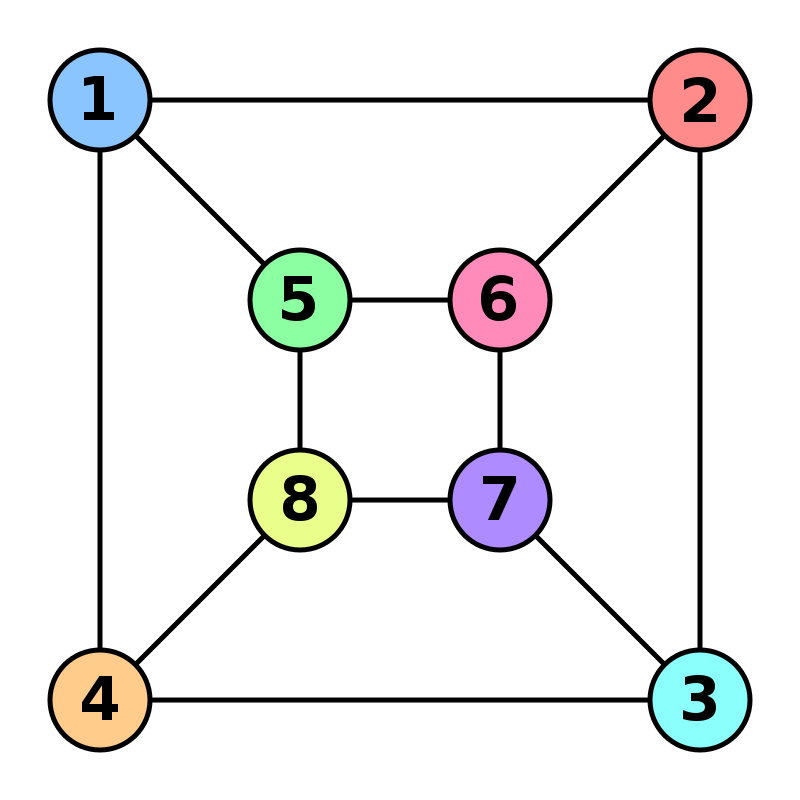
\includegraphics[scale=0.2]{figs/Graph_isomorphism_b.png}

\end{frame}

%---------------------------------------------------------


%---------------------------------------------------------
%Example of the \pause command
\begin{frame}
  \frametitle{图同构的必要不充分条件}
  \begin{center}
    \scalebox{0.8}{
      \begin{minipage}{1\linewidth}
        \begin{algorithm}[H]
        \begin{algorithmic}[1]
        \IF{$V(G) \ne V(H)$}
          \RETURN \FALSE
        \ENDIF
        \FOR{$v$ in $V(G)$ and $V(H)$}
          \STATE $L_v^0 = 1$
        \ENDFOR
        \FOR{$i=1$ to $|V(G)|$}
          \FOR{$v$ in $V(G)$ and $V(H)$}
            \STATE $L_v^i = hash (\{ L_u^{i-1} : u \in \mathcal{N}(v) \})$
          \ENDFOR
          \IF{the partition of $L_{V(G)}^{i}$ $\ne$ the partition of $L_{V(H)}^{i}$}
            \RETURN \FALSE
          \ENDIF
          \IF{no change in the partition between $L^i$ and $L^{i-1}$ of two grap}
            \STATE \textbf{break}
          \ENDIF
        \ENDFOR
        \RETURN \TRUE
        \end{algorithmic}
        \caption{Weisfeiler-Lehman Test}
        \label{alg:seq}
        \end{algorithm}
      \end{minipage}
      }
  \end{center}
\end{frame}
%---------------------------------------------------------

%---------------------------------------------------------
\begin{frame}

  \frametitle{Weisfeiler-Lehman Test 示例}
  \ctikzfig{figs/WL-1}

\end{frame}
%---------------------------------------------------------

%---------------------------------------------------------
\begin{frame}

  \frametitle{Weisfeiler-Lehman Test 示例}
  \ctikzfig{figs/WL-2}

\end{frame}
%---------------------------------------------------------

%---------------------------------------------------------
\begin{frame}

  \frametitle{Weisfeiler-Lehman Test 示例}
  \ctikzfig{figs/WL-3}

\end{frame}
%---------------------------------------------------------

%---------------------------------------------------------
\begin{frame}

  \frametitle{Weisfeiler-Lehman Test 示例}
  \ctikzfig{figs/WL-4}

\end{frame}
%---------------------------------------------------------

%---------------------------------------------------------
\begin{frame}

  \frametitle{Weisfeiler-Lehman Test 示例}
  \ctikzfig{figs/WL-5}

\end{frame}
%---------------------------------------------------------

%---------------------------------------------------------
\begin{frame}

  \frametitle{Weisfeiler-Lehman Test 示例}
  \ctikzfig{figs/WL-6}

\end{frame}
%---------------------------------------------------------

%---------------------------------------------------------
\begin{frame}

  \frametitle{Weisfeiler-Lehman Test 示例}
  \ctikzfig{figs/WL-7}

\end{frame}
%---------------------------------------------------------

%---------------------------------------------------------
\begin{frame}

  \frametitle{Weisfeiler-Lehman Test 示例}
  \ctikzfig{figs/WL-8}

\end{frame}
%---------------------------------------------------------

%---------------------------------------------------------
\begin{frame}

  \frametitle{Weisfeiler-Lehman Test 反例}
  \begin{alertblock}{Weisfeiler-Lehman Test 是图同构的必要不充分条件}
    两个同构图经过上述变换后得到的标签分布一定相同,但得到相同的标签分布只能说明两个图\textbf{可能}同构。
  \end{alertblock}
  \ctikzfig{figs/WL-ce}

\end{frame}
%---------------------------------------------------------



\section{Second section}

%---------------------------------------------------------
%Highlighting text
\begin{frame}
\frametitle{Sample frame title}

In this slide, some important text will be
\alert{highlighted} because it's important.
Please, don't abuse it.

\begin{block}{Remark}
Sample text
\end{block}

\begin{alertblock}{Important theorem}
Sample text in red box
\end{alertblock}

\begin{examples}
Sample text in green box. The title of the block is ``Examples".
\end{examples}
\end{frame}
%---------------------------------------------------------


%---------------------------------------------------------
%Two columns
\begin{frame}
\frametitle{Two-column slide}

\begin{columns}

\column{0.5\textwidth}
This is a text in first column.
$$E=mc^2$$
\begin{itemize}
\item First item
\item Second item
\end{itemize}

\column{0.5\textwidth}
This text will be in the second column
and on a second tought this is a nice looking
layout in some cases.
\end{columns}
\end{frame}
%---------------------------------------------------------


\end{document}